\chapter{Results and Discussion}
\label{chap_dis}
\section{Results}
\subsection{Cross Section of $J/\psi$ production in p-Pb collisions}
\label{sec_5_crosssection}
Figure~\ref{fig_5_xsectiony} shows the $y$ dependence of inclusive $J/\psi$ cross section. 
The blue marker shows the inclusive cross section of $J/\psi$ production at mid-rapidity (-1.37 $<$ $y_{\rm{CMS}}$ $<$ 0.43) measured in this thesis and the value is
\begin{equation}
  %\frac{d\sigma_{J/\psi}}{dy} =  946 ~\pm  ~50.1 ~\rm{(stat)} ~\pm 54 ~\rm{(uncorr.~syst)} ~\pm 32 ~\rm{(corr.~syst)}~\mu \rm{b}
%  \frac{d\sigma_{J/\psi}}{dy} =  946 ~\pm  ~50.1 ~\rm{(stat)} ~\pm 63 ~\rm{syst}~\mu \rm{b}
       \frac{d\sigma_{J/\psi}}{dy} =   930 ~\pm 83 ~\rm{(stat)} ~\pm ~59 ~\rm{(uncorr. syst)} ~\pm~ 31\rm{(corr. syst)} ~\mu  \rm{b}
\end{equation}
The latter 2 components express the correlated and uncorrelated systematic uncertainties with respect to the dimuon ($\mu^{+}\mu^{-}$) decay measurement, respectively.
The red marker shows the inclusive $J/\psi$ cross section measured via dimuon decay channel with the ALICE muon arm~\cite{bib_alicemuon}.
\begin{figure}[!h]
  \centering
  \includegraphics[width=12cm]{chap5/figure/CrossSection/JpsiCrossSection_MB_Y_tw.eps}
  \caption{$y$ dependence of the Cross section in p-Pb collisions at $\sqrt{s_{NN}}=$ 5.02 TeV. 
    The blue marker shows my results in mid-rapidity. 
    The red marker show the measured cross section via dimuon decay channel in ALICE. 
    The open square shows the uncorrelated systematic uncertainty and the shaded band shows the partially or fully correlated systematic uncertainties. 
  }
  \label{fig_5_xsectiony}
\end{figure}

%In this figure, the fully correlated and the partially correlated uncertainties are following, 
%Since the systematic uncertainty of the normalization by the minimum event cross section $\sigma_{V0}$ is partially or fully correlated between dielectron and dimuon analysis, this uncertainty is expressed as the shaded band in Fig~\ref{fig_5_xsectiony} 
%The open square and the shaded band show the uncorrelated and partially and fully correlated systematic uncertainties, respectively. 
The shaded band of the muon measurements expresses the partially correlated or fully correlated uncertainties.
Partially correlated uncertainty is caused by the difference of the LHC run mode 'p-Pb' and 'Pb-p' defined in Section.~\ref{sec_3_runcondition}.
The central and forward rapidity measurements are performed in the 'p-Pb' mode. 
On the other hand, the backward rapidity measurement is performed in the 'Pb-p' mode. 
Therefore the minimum bias cross section $\sigma_{V0}$ is different each other but their systematic uncertainties are partially correlated. 
In the muon measurement, the sources of the partially correlated and correlated uncertainties are as follows. 
\begin{description}
	\item{- Partially correlated uncertainty:}  Minimum bias cross section
	\item{- Correlated uncertainty:}  Branching ratio
\end{description}
In case of the electron analysis, the minimum bias cross section and the branching ratio are correlated with respect to the muon measurement and expressed by the blue shaded band. 

Figure~\ref{fig_5_xsectionpt} shows the invariant cross section of $J/\psi$ production as a function of $p_{\rm{T}}$. 
The open square shows the uncorrelated systematic uncertainty and the shaded bands show the correlated uncertainty which comes from the uncertainties of $\sigma_{V0}$ and branching ratio of the dielectron decay channel. 
The values of the cross section, statistical uncertainty, and systematic uncertainty of $J/\psi$ cross section are summarized in Table.~\ref{table_5_xsection}.
\begin{figure}[!h]
  \centering
  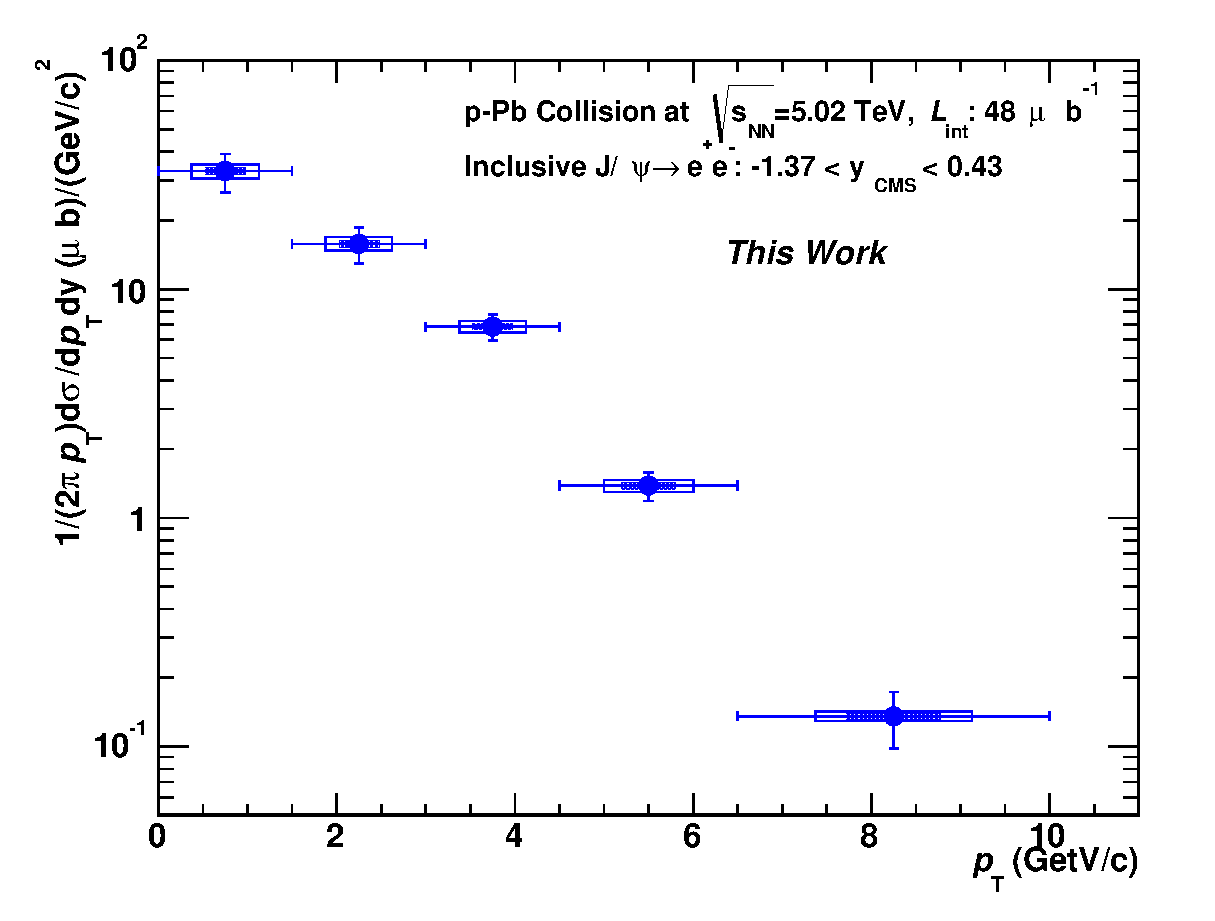
\includegraphics[width=12cm]{chap5/figure/CrossSection/JpsiInvCrossSection_MB_Pt_bin2_tw.eps}
  \caption{
    Invariant cross section as a function of $p_{\rm{T}}$ in p-Pb collisions at $\sqrt{s_{NN}}=$ 5.02 TeV.
    The open square shows the uncorrelated systematic uncertainty and the shaded band shows the correlated systematic uncertainties. 
  }
  \label{fig_5_xsectionpt}
\end{figure}
\begin{table}[!h]
  \centering
  \begin{tabular}{c|c} \hline
    $p_{\rm{T}}$ (GeV/$c$)  bin & $d\sigma_{J/\psi}/dp_{\rm{T}}dy$ $\pm$ stat $\pm$ uncorr. syst $\pm$  corr.syst ($\mu$b)\\ \hline
    0.0 - 1.5                     & 154 $\pm$ 30 $\pm$ 11 $\pm$ 5  \\
    1.5 - 3.0                   & 223 $\pm$ 40 $\pm$ 17 $\pm$ 7  \\
    3.0 - 4.5                   & 162 $\pm$ 21 $\pm$ 11 $\pm$    \\
    4.5 - 6.5                   & 47 $\pm$ 7 $\pm$ 3 $\pm$ 2    \\
    6.5 - 10.0                  & 7.0 $\pm$ 2.0 $\pm$  0.6 $\pm$ 0.2                        \\ \hline
  \end{tabular}
  \caption{Summary of the inclusive $J/\psi$ cross section and their uncertainties in p-Pb collisions at $\sqrt{s_{NN}}=$5.02 TeV.}
  \label{table_5_xsection}
\end{table}
From the cross section spectrum, the mean $p_{\rm{T}}$ of $J/\psi$ is $2.815\pm0.095(\rm{stat})\pm0.01(\rm{syst})$ (GeV/$c$). 
Compared to the interpolated mean $p_{\rm{T}}$ in pp collision at $\sqrt{s}=5.02$ TeV in Table~\ref{table_4_pprefvalue}, it is consistent within the uncertainty. 

\subsection{$R_{\rm{pPb}}$ of Inclusive $J/\psi$ production in p-Pb Collisions}
The nuclear modification factor $R_{\rm{pPb}}$ is calculated with the yield of $J/\psi$  in p-Pb collisions and interpolated pp as shown in Eq.~\ref{eq_4_rppb}.
Figure~\ref{fig_5_rppby} shows the $y$ dependence of the inclusive $J/\psi$ $R_{\rm{pPb}}$. 
The red marker shows the results of dimuon decay $J/\psi$ at forward and backward rapidity region with the ALICE muon arm.  
The inclusive $J/\psi$ $R_{\rm{pPb}}$ measured in this thesis at mid-rapidity ($-1.37 < y< 0.43$) is
\begin{equation}
  R_{\rm{pPb}} = \rm{0.74 ~\pm ~0.07 ~(stat) ~\pm ~0.13 ~(uncorr.~syst) ~\pm ~0.03 ~(corr.~syst) }
\end{equation}
The latter 2 components express the correlated and uncorrelated systematic uncertainties with respect to the dimuon decay measurement, respectively. 
The correlated systematic uncertainty with respect to dimuon measurement comes from the common normalization by the thickness function $T_{\rm{pPb}}$.
The significant suppression of $J/\psi$ production is observed compared to pp collisions due to the nuclear matter effects in p-Pb collisions. 
In the dimuon measurement,  the partially correlated and the fully correlated are defined as follows. 
\begin{description}
	\item{- Partially correlated uncertainty:} Interpolation of rapidity dependence of pp reference cross section. 
	\item{- Correlated uncertainty:}  Thickness function ($T_{\rm{pPb}}$), Interpolation of pp reference cross section from the measured data.
\end{description} 
The integrated forward (2.03 $<y<$ 3.53) and backward (-4.46 $<y<$ -2.96) $R_{\rm{pPb}}$ is 
0.70 $\pm$ 0.01 (stat) $\pm$ 0.06 (uncorr. syst) $\pm$ 0.03 (part. corr. syst) $\pm$ 0.03 (corr. syst) and 
1.08 $\pm$ 0.01 (stat) $\pm$ 0.09 (uncorr. syst) $\pm$ 0.03 (part. corr. syst) $\pm$ 0.04 (corr. syst) 
, respectively.
The mid-rapidity result shows the same level of suppression as the result of forward rapidity region where partons with smaller $x$($\propto \rm{e}^{-y}$) are dominant and stronger suppression is expected due to the modification of nPDF. 
\begin{figure}[!h]
  \centering
  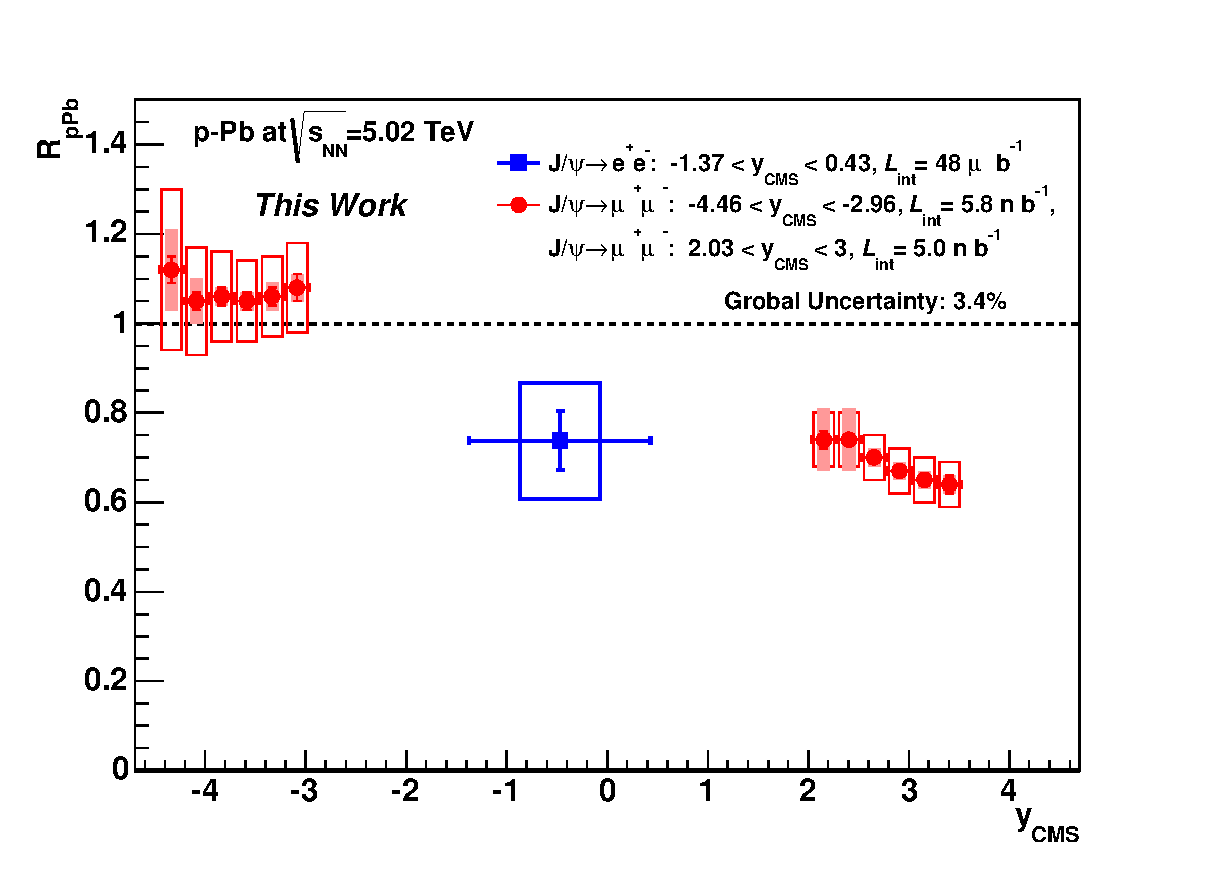
\includegraphics[width=12cm]{chap5/figure/RpPb/RpPb_MB_y_bin2_tw.eps}
  \caption{$R_{\rm{pPb}}$ as a function of $y$ in p-Pb collisions at $\sqrt{s_{NN}}=$ 5.02 TeV.}
  \label{fig_5_rppby}
\end{figure}

Figure~\ref{fig_5_rppbpt} shows the $p_{\rm{T}}$ dependence of the inclusive $J/\psi$ $R_{\rm{pPb}}$. 
The black band around the right axis shows the uncertainty of the normalization with $T_{\rm{pPb}}$ and $d\sigma_{J/\psi}/dy$. 
The suppression $\sim 2.4\sigma$ is seen at the low and intermediate $p_{\rm{T}}$ bins ($p_{\rm{T}}=$ 1.5-3 GeV/$c$).
Above 5 GeV/$c$, no modification is observed within the uncertainties.  
The values of $R_{\rm{pPb}}$ and uncertainties of the inclusive $J/\psi$ production are summarized in Table~\ref{table_5_rppb}.
\begin{figure}[!h]
  \centering
  \includegraphics[width=12cm]{chap5/figure/RpPb/RpPb_MB_Pt_bin2_tw.eps}
  \caption{$R_{\rm{pPb}}$ as a function of $p_{\rm{T}}$ in p-Pb collisions at $\sqrt{s_{NN}}=$ 5.02 TeV.}
  \label{fig_5_rppbpt}
\end{figure}

\begin{table}[!h]
  \centering
  \begin{tabular}{c|c} \hline
    $p_{\rm{T}}$ bin (GeV/$c$)  & $R_{\rm{pPb}}\pm stat \pm uncorr. syst \pm corr. syst$ \\ \hline
    0.0 - 1.5 & 0.83 $\pm$ 0.15 $\pm$ 0.08 $\pm$ 0.14 \\
    1.5 - 3.0    & 0.62 $\pm$ 0.11 $\pm$ 0.05 $\pm$ 0.10 \\
    3.0 - 4.5  & 0.72 $\pm$ 0.11 $\pm$ 0.06 $\pm$ 0.12 \\
    4.5 - 6.5 & 1.00 $\pm$ 0.13 $\pm$ 0.12 $\pm$ 0.17 \\
    6.5 - 10.0 & 0.83 $\pm$ 0.18 $\pm$ 0.14 $\pm$ 0.14 \\ \hline
  \end{tabular}
  \caption{Summary of the inclusive $J/\psi$ $R_{\rm{pPb}}$ and the uncertainties in p-Pb collisions at $\sqrt{s_{NN}}=$5.02 TeV.}
  \label{table_5_rppb}
\end{table}

\clearpage
\section{Discussion}
\subsection{Comparison with the Quantitative Model Calculation}
The results are compared to the several models including different nuclear matter effects such as the modification of parton nPDF, coherent energy loss model, and gluon saturation. 
The theoretical models discussed in this thesis are 
\begin{description}
\item{NLO Color Evaporation Model with  EPS09 nPDF~\cite{bib_shadow}}  \\ \mbox{}
This calculation includes the modification of nPDF expected by EPS09 parametrization. 
The main uncertainty of EPS09 band comes the shadowing parametrization.
Since Deep Inelastic Scattering (DIS) is not sensitive to gluon PDF, nPDF parametrization in EPS09 uses the inclusive pion production in d+Au at RHIC~\cite{bib_daupion}. 
However the uncertainty has still large band in small and intermediate $Q^{2}$ as shown in Fig.~\ref{fig_2_pdf}.
$J/\psi$ production from $c\bar{c}$ is described by the NLO color evaporation model (CEM) in this calculation. 

\item{EPS09 Leading-Order Calculation~\cite{bib_shadowlo}} \\ \mbox{}
This calculation is based on the $2\rightarrow 2$ process like $g+g\rightarrow J/\psi + g$. 
The motivation of this calculation comes from the leading order calculation of the color singlet model (CSM) which predicts $2\rightarrow2$ process is dominant in low $p_{\rm{T}}$ $J/\psi$ production. 
Relatively small absorption cross section $\sigma_{abs}$ (1.5 mb and 2.8 mb) are also considered as the effect of unknown $c\bar{c}$ breakup. 
In comparison to data, one has to be careful for the dependence of the factorization scale $\mu_{F}$~\cite{bib_shadowlo}. 
The results with central set of EPS09 leading-order calculation have the scale uncertainty as shown in Fig.~\ref{fig_5_eps09louncertainty}.
\begin{figure}[!h]
  \centering
  \includegraphics[width=8cm]{chap5/figure/ModelComp/epslouncertainty.png}
  \caption{EPS09 leading-order scale uncertainty~\cite{bib_shadowlo}. }
  \label{fig_5_eps09louncertainty}
\end{figure}

\item{Parton Energy Loss in the Normal Nuclear Matter~\cite{bib_jpsipaeloss}} \\ \mbox{} 
This calculation takes into account the coherent energy loss in the nuclei. 
The detail of this calculation is described in Section.~\ref{sec_2_eloss}. 
The transport coefficient includes the effect of gluon density evolution with $\hat{q}(x)\sim\hat{q}_{0}(\cfrac{10^{-2}}{x})^{0.3}$.
$\hat{q}_{0}$ is the only parameter in this calculation. 
The calculation is performed with two $\hat{q}$ parametrization ($\hat{q}_{0}=0.05 ~\rm{GeV^{2}/fm}$ and 0.075 \rm{GeV^{2}/\rm{fm}}$) in four nPDF assumption(pp parametrization, DSSZ, EPS09 nPDF, and Gluon Saturation) as shown in Fig.~\ref{fig_2_paeloss}. 

\item{Color Glass Condensate Framework Calculation~\cite{bib_jpsisaturation,bib_cgc,bib_cgc2}} \\ \mbox{}
At forward rapidity, calculations are performed using CGC framework for the nucleus probed at small $x$ and the collinear framework with proton PDF probed at large $x$.  
In the Ref~\cite{bib_jpsisaturation}, nPDF is calculated with the Balitsky-Kovchegov (BK) equation including the running coupling corrections (rcBK equation).  CEM is adopted in the $J/\psi$ formation.  
The main systematic uncertainty of the calculation comes from the uncertainties of $Q_{s}^{2}$ and charm quark mass. 
Other calculations adopting CEM and NRQCD model are also performed.
\end{description}

Figure~\ref{fig_5_rppbyvsshadow} shows the comparison of the $y$ dependence of $R_{\rm{pPb}}$ with the shadowing model calculation. 
At mid-rapidity, both models of NLO and LO EPS09 parametrization are consistent with the data within the uncertainties. 
Despite the large global uncertainty, EPS09 leading-order calculation describes the qualitatively description of the $y$ dependence. 
The NLO shadowing shows the less suppression compared to the data as rapidity increasing. 
At mid-rapidity and forward rapidity, both of calculations don\rq{}t show the strong rapidity dependence although the magnitudes of the central points are different.  
\begin{figure}[!h]
  \centering
  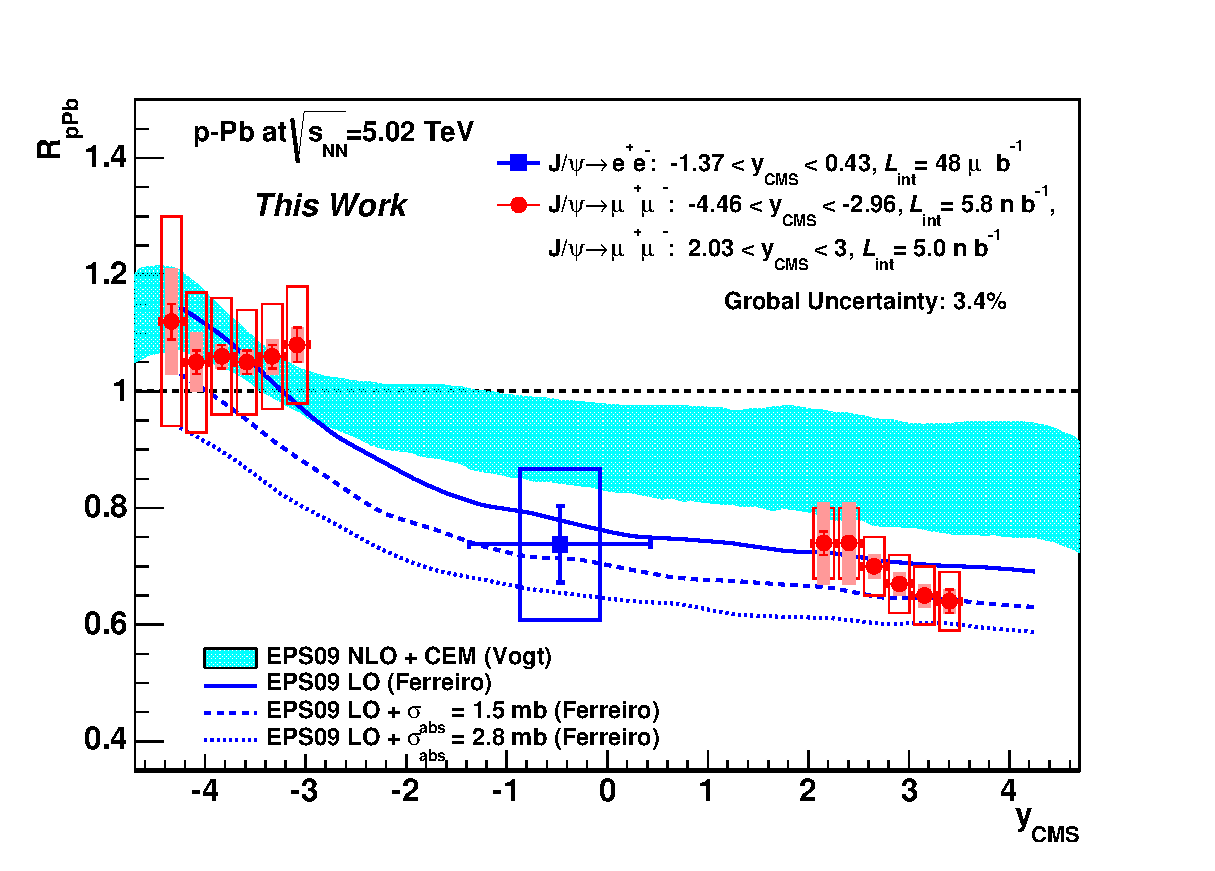
\includegraphics[width=10cm]{chap5/figure/ModelComp/JpsiRpPb_shadowing_y.eps}
  \caption{Comparison of the $y$ dependence with the shadowing model calculation of $J/\psi$ $R_{\rm{pPb}}$ in p-Pb collisions at $\sqrt{s_{NN}}=$ 5.02 TeV~\cite{bib_shadow,bib_shadowlo}.}
  \label{fig_5_rppbyvsshadow}
\end{figure}
The recent progress of nCTEQ15 parametrization by global fit with CTEQ PDF also shows the same trend of $R^{\rm{Pb}}_{g}$ with stronger suppression than EPS09 as shown in Fig.~\ref{fig_5_ncteq}~\cite{bib_ncteq15,bib_cteq,bib_ncteq15shadow}. 
The feature of $R^{\rm{Pb}}_{g}$ calculated by the several nPDFs at small $x$ is qualitatively similar to the weak rapidity dependence of $R_{\rm{pPb}}$ at mid-rapidity and forward rapidity.  
Due to the stronger suppression, calculation based on nCTEQ15 might give a better description of the data. 
\begin{figure}[!h]
  \centering
  \includegraphics[width=10cm]{chap5/figure/ModelComp/ncteq15.png}
  \caption{$R_{g}^{Pb}(x, Q=3\rm{GeV})$ for DSSZ, EPS09, and nCTEQ15 nPDFs~\cite{bib_ncteq15shadow}.}
  \label{fig_5_ncteq}
\end{figure}

Under the assumption that $2\rightarrow1$ process is dominant, the prediction based on nPDFs is almost identical value of $R_{g}^{\rm{Pb}}$ at $x= \frac{\sqrt{\langle p_{\rm{T}}\rangle^{2} +m_{J/\psi}^{2}}}{\sqrt{s}}e^{-y}$ and $Q=\sqrt{\langle p_{\rm{T}}\rangle^{2} + m_{J/\psi}^{2} }$. 
The $2\rightarrow 2$ case is also discussed in Ref.~\cite{bib_shadowf}.
If we take the mean $p_{\rm{T}}$ as the value in Section~\ref{sec_5_crosssection}, the mid-rapidity measurement probes $x=5.4\times 10^{ー4}$-$3.3\times10^{-3}$ and $Q^{2}\sim18$ $\rm{GeV}^{2}$. 
 If other nuclear matter effects are neglected, $R_{g}^{Pb}$ is identical $R_{\rm{pPb}}$ $\sim0.74 \pm 0.15$.  
 The effect of nuclear absorption in the leading-order EPS09 calculation suppress the yield by a factor 15\% at $y\sim0$. 
 The coherent energy loss also expects to suppress the yield by a factor 20\% if no modification of nPDF is assumed. 
Therefore if the other suppression is considered by a factor 15-20\%, the central point of $R_{g}^{\rm{Pb}}$ is 0.87$\sim$0.92.
Figure~\ref{fig_5_xcover} shows the $x$ coverage of parton in Pb for $2\rightarrow 1$ process as a function of $J/\psi$ $p_{\m{T}}$ in p-Pb collisions and Pb-Pb collisions at LHC. 
Since the probing $Q^{2}$ is expressed as $p_{\rm{T}, J/\psi}^{2} + m_{J/\psi}^{2}$, the mean $Q^{2}$ in 0-1.5 GeV/$c$ bin of $J/\psi$ $p_{\rm{T}}$ is $\sim 10.1 \rm{GeV^{2}}$ and the expected $R_{g}^{Pb}$ is 0.84 $\pm$ 0.22. 
It is compatible to the result of EPS09 calculation at $Q^{2}=10$ $\rm{GeV}^{2}$ in Fig.~\ref{fig_2_pdf}.
\begin{figure}[!h]
  \centering
  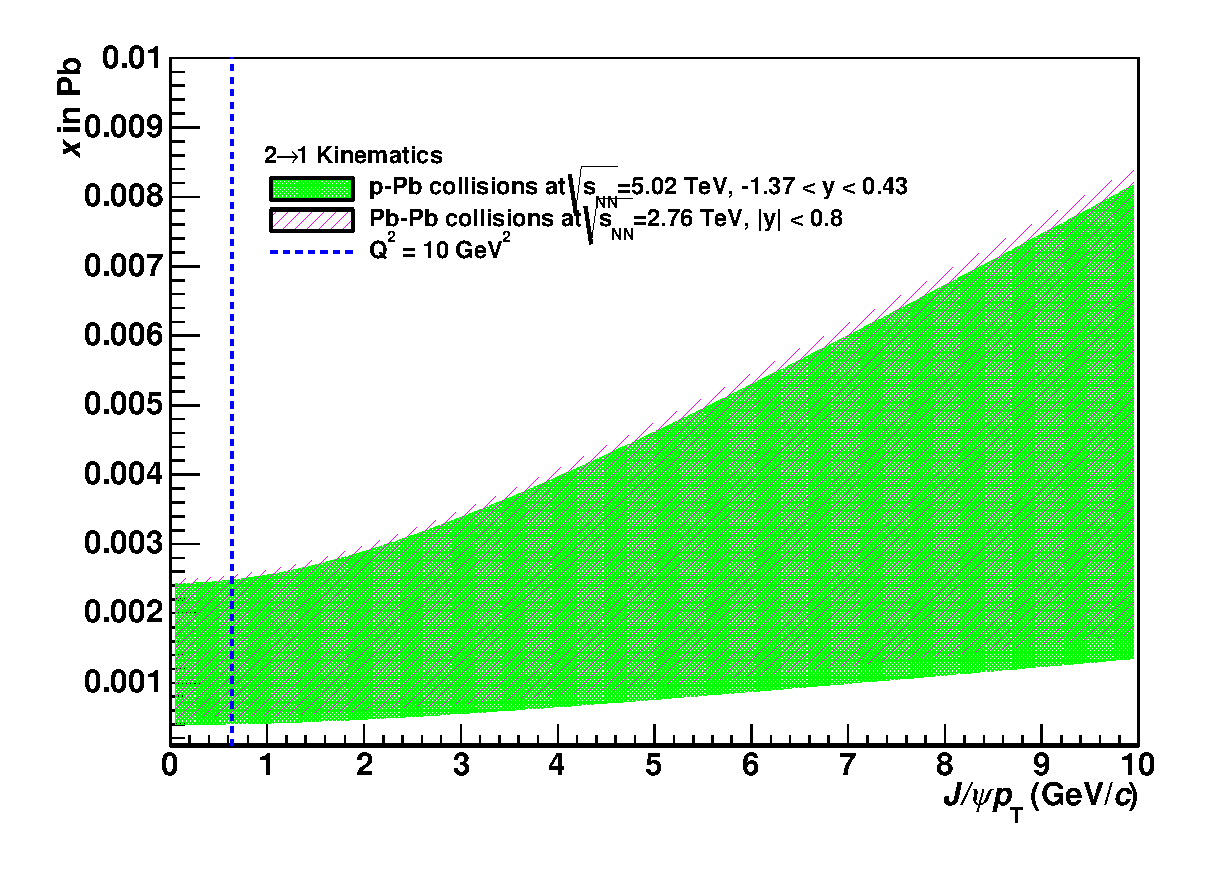
\includegraphics[width=8cm]{chap5/figure/xcover/xcoverageofjpsi.eps}
  \caption{$x$ coverage in Pb of the $J/\psi$ measurement at mid-rapidity in p-Pb collision at $\sqrt{s_{NN}}=5.02$ TeV and Pb-Pb collisions at $\sqrt{s_{NN}}=$ 2.76 TeV in case of $2\rightarrow1$ kinematics. }
  \label{fig_5_xcover}
\end{figure}


Figure~\ref{fig_5_rppbyvseloss} shows the comparison of the $y$ dependence with the coherent energy loss calculation of $J/\psi$ $R_{\rm{pPb}}$~\cite{bib_jpsipaeloss}.
\begin{figure}[!h]
  \centering
  \includegraphics[width=10cm]{chap5/figure/ModelComp/JpsiRpPb_eloss_y.eps}
  \caption{Comparison of the $y$ dependence with the coherent energy loss calculation of $J/\psi$ $R_{\rm{pPb}}$ in p-Pb collisions at $\sqrt{s_{NN}}=$ 5.02 TeV~\cite{bib_jpsipaeloss}.}
  \label{fig_5_rppbyvseloss}
\end{figure}
The solid and dashed curves show the coherent energy loss calculation with EPS09 nPDF and the proton PDF, respectively.
Taking shadowing parametrization means the initial number of $c\bar{c}$ pairs becomes smaller compared to the case taking the proton PDF. 
Coherent energy loss model with typical $\hat{q}$ shows the reasonable description of the rapidity dependence qualitatively. 
The calculation with proton PDF parametrization shows the better agreement with the results although no modification of nPDF is assumed.  
%From the comparison between data and the coherent energy loss with EPS09 parametrization,  $\hat{q}$ in coherent energy loss process is expected smaller than $\hat{q}<$0.055 $\rm{GeV^{2}/fm}$.

Figure~\ref{fig_5_rppbyvscgc} shows the comparison of the $y$ dependence with the CGC calculation of $J/\psi$ $R_{\rm{pPb}}$ in p-Pb collisions~\cite{bib_jpsisaturation,bib_cgc,bib_cgc2}.
The discrepancy of the calculation in Ref.~\cite{bib_jpsisaturation} is argued that it might be caused by the geometrical effects within less than 2$\sigma$.
 The other calculation with CEM introduces the impact parameter dependence and shows the better description of the data. 
 CGC+NRQCD also shows the consistency with the data within the finite uncertainties.  
\begin{figure}[!h]
  \centering
  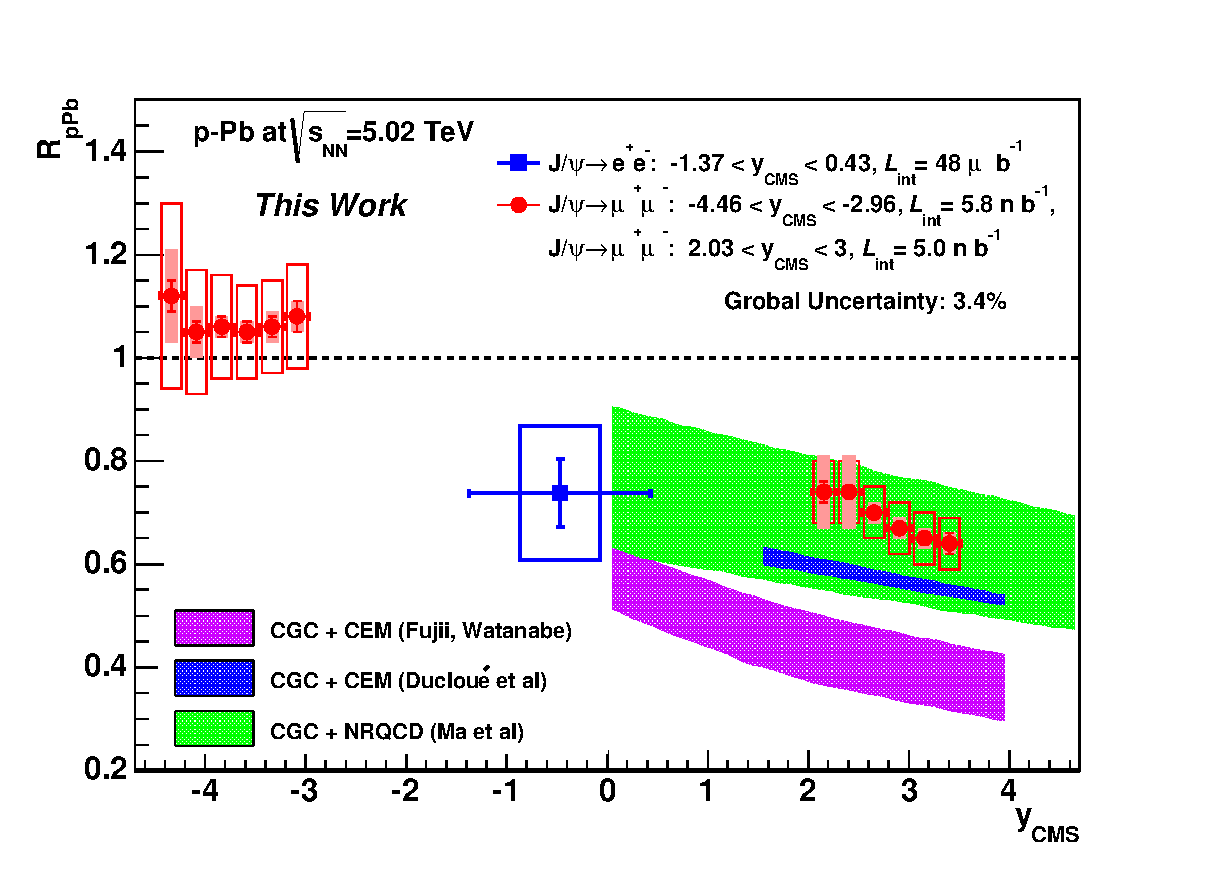
\includegraphics[width=10cm]{chap5/figure/ModelComp/JpsiRpPb_cgc_y.eps}
  \caption{Comparison of the $y$ dependence with the CGC calculation of $J/\psi$ $R_{\rm{pPb}}$ in p-Pb collisions at $\sqrt{s_{NN}}=$ 5.02 TeV~\cite{bib_jpsisaturation,bib_cgc,bib_cgc2}.}
  \label{fig_5_rppbyvscgc}
\end{figure}

Figure~\ref{fig_5_rppbm} shows the comparison of the $p_{\rm{T}}$ dependence between the measured $R_{\rm{pPb}}$ and the color evaporation model with EPS09 nPDF at mid-rapidity. 
There is a consistency within the large global uncertainty. 
Figure~\ref{fig_5_rppbm3} shows the comparison of the $p_{\rm{T}}$ dependence between the measured $R_{\rm{pPb}}$ and the model calculations. 
The red, green, and magenta bands show the calculation based on gluon saturation with CGC framework, coherent energy loss with EPS09 nPDF parametrization, and coherent energy loss with the proton PDF parametrization.
The coherent energy loss calculation shows the agreement with the data within the uncertainty. 

As a summary of the model comparison to the data, the coherent energy loss model shows the reasonable description of the both of $y$ and $p_{\rm{T}}$ dependence. 
On the other hand, although there is still model dependence of the suppression strength, $R_{g}^{\rm{Pb}}$ calculated with several nPDFs shows the weak $x$ dependence at small $x$ and it is qualitatively consistent with the rapidity dependence of the data.  
CGC calculations might describe the data at forward $J/\psi$ production. 
However the uncertainties are still large for both data and model calculation. 
The main sources of the uncertainties of the experimental data are the statistical uncertainty and the uncertainty of the interpolated pp reference spectra. 
To achieve high precision, the reduction of these uncertainties are needed.  
\begin{figure}[!h]
  \centering
  \includegraphics[width=10cm]{chap5/figure/ModelComp/RpPb_MB_wModelEPS_Pt_bin2_tw.eps}
  \caption{Comparison of the $p_{\rm{T}}$ dependence between the measured $R_{\rm{pPb}}$ and the color evaporation model with EPS09 nPDF in p-Pb collisions at $\sqrt{s_{NN}}=$ 5.02 TeV.}
  \label{fig_5_rppbm}
\end{figure}

\begin{figure}[!h]
  \centering
  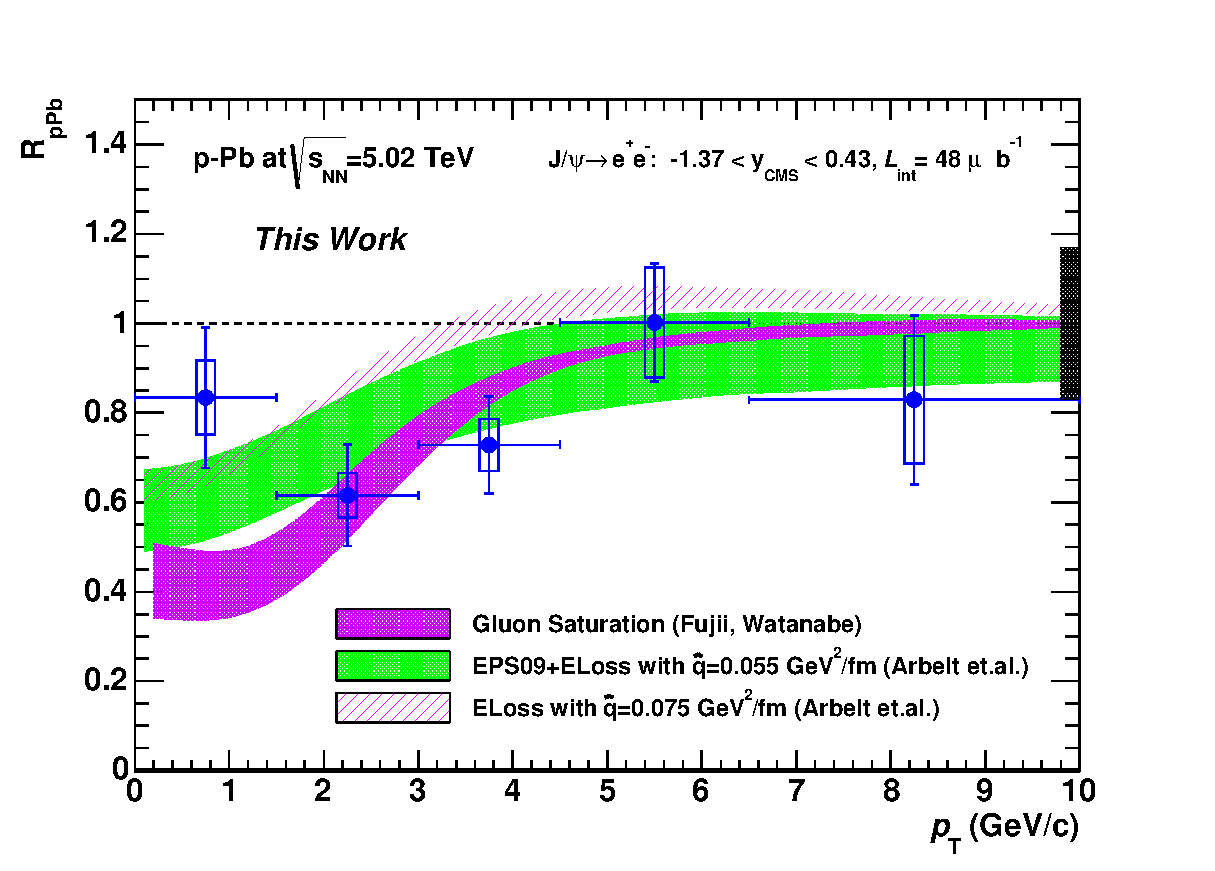
\includegraphics[width=10cm]{chap5/figure/ModelComp/RpPb_MB_w3Model_Pt_bin2_tw.eps}
  \caption{Comparison of the $p_{\rm{T}}$ dependence between the measured $R_{\rm{pPb}}$ and the model calculations in p-Pb collisions at $\sqrt{s_{NN}}=$ 5.02 TeV. The red, green, and magenta bands show the calculation based on gluon saturation with CGC framework, coherent energy loss with EPS09 nPDF parametrization, and coherent energy loss with pp PDF parametrization. }
  \label{fig_5_rppbm3}
\end{figure}

\clearpage
\subsection{Comparison to A-A collisions}
%\subsection{Comparison to A-A collisions and Extraction of QGP Effects}
%\subsection{Factorization of the Normal Nuclear Matter Effects}
%The nuclear modification factor in heavy ion collisions ($R_{\rm{AA}}$) can be divided into 3 parts, $R_{\rm{AA}}=R_{\rm{AA}}^{Init}\times R_{\rm{AA}}^{QGP} \times R_{\rm{AA}}^{Had}$. 
%$R_{\rm{AA}, init}$ expresses the nuclear modification factor of initial parton-parton scattering. 
%$R_{\rm{AA}, QGP}$ and $R_{\rm{AA, Had}}$ express the nuclear modification factor affected by QGP and the hadron gas phase, respectively. 
$J/\psi$ production in the initial parton-parton scattering($gg\rightarrow J/\psi+X$) is expressed by
\begin{equation}
  \sigma_{\rm{PbPb} \rightarrow J/\psi X} = \Sigma_{i, j, k_{cc}} f_{i}^{\rm{Pb}}(x_{i}) ~\times ~\sigma_{i+j\rightarrow k_{cc}} ~\times ~f_{j}^{\rm{Pb}}(x_{j}) ~\times ~\sigma_{k_{cc}\rightarrow J/\psi X}
\end{equation}
%A simple approximation to determine the normal nuclear matter effects is valid in the gluon shadowing dominant region~\cite{bib_shadow}.
To discuss normal nuclear matter effects in Pb-Pb collisions from the experimental results, we consider the following assumption,  
\begin{description}
	\item{-}  $2\rightarrow 1$ process is dominant. 
	\item{-}  The effect of nPDF modification is dominant and other effects are small. 
\end{description}
In this case, the $x$ coverage of p-Pb collisions and Pb-Pb collisions  is almost same and the difference is about 6\% as shown in Fig.~\ref{fig_5_xcover}.
The latter assumption leads the modification in $R_{\rm{pPb}}$ is only affected by nPDF and $R_{\rm{pPb}}$ is identical with $R_{g}^{\rm{Pb}}$ at same $x$ and $Q$~\cite{bib_shadow}.
To estimate the strength of initial normal nuclear matter effects in Pb-Pb collisions, the convolution of $R_{\rm{pPb}}$ is calculated as the normal nuclear matter effects in $R_{AA}$~\cite{bib_shadowf},  
\begin{eqnarray}
	R_{AA, init} = & R_{\rm{pPb}}(y, b_{1})\times R_{\rm{pPb}}(-y, b_{2})
  %R_{AA, init}|_{y\sim 0} & = & R_{pPb}|_{y \sim 0} \times R_{pPb}|_{y\sim0} \nonumber \\
%  R_{AA, init}|_{forward} & = & R_{pPb}|_{forward} \times R_{pPb}|_{backward}
\end{eqnarray}
where $b_{1}$ and $b_{2}$ is the impact parameter of incident nucleons with respect to target nuclei.  
This is a laugh estimation but the estimated $R_{AA, init}$ in Au-Au collision at RHIC is extracted with this approximation and provides the indication of $J/\psi$ suppression as shown in Fig.~\ref{fig_2_cnmraa} and \ref{fig_2_saavse}~\cite{bib_daucorr}.
The similar calculation in $2\rightarrow2$ process is discussed in Ref.\cite{bib_shadowf}. 
The rapidity dependence is different but the same results are obtained in  $2\rightarrow1$ and $2\rightarrow2$ process at mid-rapidity region.
\begin{figure}[!h]
  \centering
  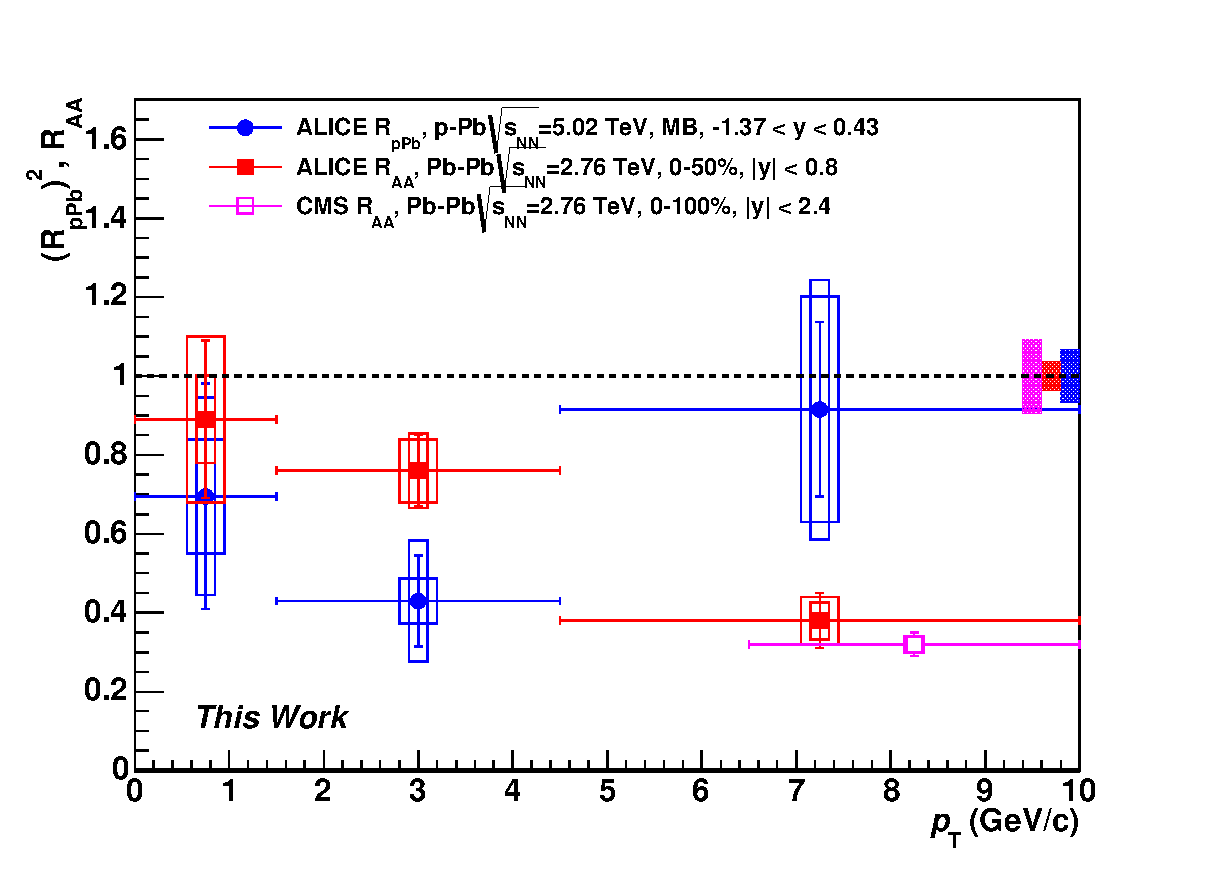
\includegraphics[width=10cm]{chap5/figure/SAA/JpsiRpbRpb_bin2_tw.eps}
  \caption{
  Comparison of $R_{AA}$ and $(R_{\rm{pPb}})^{2}$ in ALICE. The data points of Pb-Pb collisions are take from ~\cite{bib_alicejpsiraamid}. 	
  }
  \label{fig_5_rppbrppb}
\end{figure}
Figure~\ref{fig_5_rppbrppb} shows the comparison of $R_{AA}$ in 0-50\% centrality and square of ($R_{\rm{pPb}})^{2}$ collision in at mid-rapidity.
The Pb-Pb data shows a smooth suppression in all $p_{\rm{T}}$ region but the direct comparison to the ($R_{\rm{pPb}})^{2}$ indicates two features. 
First point is a clear suppression above $p_{\rm{T}}>$ 4.5 GeV/$c$. 
Therefore the suppression at high $p_{\rm{T}}$ in Pb-Pb collisions is thought as QGP effects.
%%This suppression suggests the indication of QGP effects. 
The second point is the significant enhancement at lower $p_{\rm{T}}$. 
It suggests that the suppression in $R_{AA}$ is not QGP matter effects but the normal nuclear matter effects. 
According to model calculations, regeneration enhancement is dominant below 5 GeV/c at the mid-rapidity  
because the regenerated charm quarks are thermalized and their momentum spectrum becomes very soft~\cite{bib_recomodel}. 
Therefore this is expected to be due to the enhancement of $J/\psi$ regeneration in QGP. 
As a next step, survival fraction $S_{AA}$ is extracted as follows. 
\begin{equation}
  	S_{AA}  = \cfrac{R_{AA}}{R_{AA, init}}
 \end{equation} 
Figure~\ref{fig_5_saa} shows the survival fraction $S_{AA}$. 
%The propagation of the correlated.  At higher $p_{T}$, this can be thought as the pure signal of color screening. 
%Due to the fact that color screening does not have clear $p_{\rm{T}}$ dependence, 
%the strength of color screening is extrapolated from high $p_{T}$ assuming the flat shape. 
%After subtracting the surviving $J/\psi$, the rest is thought only regenerated $J/\psi$ 
%The signals of lower 2 bins are merged by the weighted mean and the enhancement factor is determined. 
\begin{figure}[!h]
  \centering
  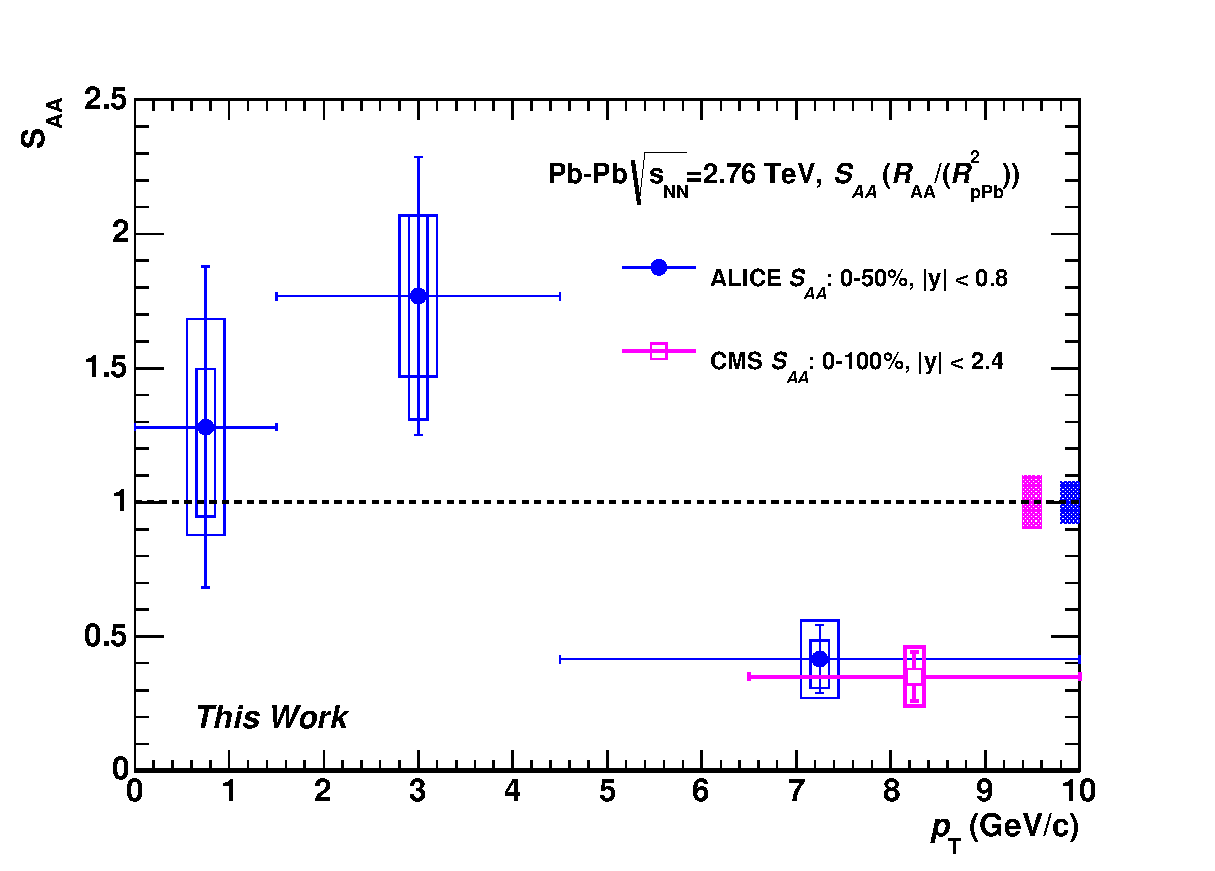
\includegraphics[width=10cm]{chap5/figure/SAA/JpsiSAA_wCMS_bin2_tw.eps}
  \caption{
	Survival fraction ($S_{AA}$) of $J/\psi$ production in Pb-Pb collisions. 
    }
  \label{fig_5_saa}
\end{figure}
The significant enhancement is seen in 1.5-4.5 GeV/$c$ bin. 
The measured value of $S_{AA}$ is 1.77 $\pm$ 0.52 (stat) $\pm$  0.30 (uncorr. syst) $\pm^{0.45}_{0.30}$ (corr. syst).
On the other hand, the measured $S_{AA}$ is 0.41 $\pm$  0.12 (stat)$ \pm$ 0.14 (uncorr. syst) $\pm$ $^{0.1}_{0.07}$ (corr. syst). 
Even though the surviving $J/\psi$ from initial collisions exists at low $p_{\rm{T}}$, this fraction is expected to be same order with high $p_{\rm{T}}$ $J/\psi$. 
Therefore newly-formed $J/\psi$ in QGP is expected to be dominant or compatible to the initial $J/\psi$ at low $p_{\rm{T}}$.   
It is qualitatively consistent with the color screening and regeneration pictures of $J/\psi$ production in QGP. 
%%
%%%%%%Therefore the same amount $J/\psi$  is regenerated in QGP compared to the production of the initial hard process.



%\begin{figure}[!h]
%  \centering
%  \includegraphics[width=12cm]{chap5/figure/AA/JpsiRpPbsqvsRAA_0-40_bin2.eps}
%  \caption{Inclusive $J/\psi$ $R_{\rm{AA}}$ in Pb-Pb collisions at $\sqrt{s_{NN}}=$2.76 TeV in 0-40\% centrality and the product of the inclusive $J/\psi$ $R_{\rm{pPb}}$ in p-Pb collisions. The data points of $R_{\rm{AA}}$ are taken from~\cite{bib_jpsiraaalice}}
%  \label{fig_5_rppby}
%\end{figure}




